\documentclass[acmlarge, anonymous]{acmart}

\usepackage{booktabs} % For formal tables
\usepackage[utf8]{inputenc}
\usepackage[ngerman]{babel}

% Copyright
\setcopyright{none}
%\setcopyright{acmcopyright}
%\setcopyright{acmlicensed}
%\setcopyright{rightsretained}
%\setcopyright{usgov}
%\setcopyright{usgovmixed}
%\setcopyright{cagov}
%\setcopyright{cagovmixed}

\acmDOI{ph342m91337}

% ISBN
\acmISBN{123-4567-24-567/08/06}

%Conference
\acmConference[]{Agententechnologien}{2018}{Berlin, Deutschland}
\acmYear{2018}
\copyrightyear{2018}

%\acmBadgeL[http://ctuning.org/ae/ppopp2016.html]{ae-logo}
%\acmBadgeR[http://ctuning.org/ae/ppopp2016.html]{ae-logo}


\begin{document}
\title{Augmentierung der DIGINET-PS durch Agententechnologien}

%\author{Johannes Gräger}
%\affiliation{%
%  \institution{TU Berlin}
%  \city{Berlin}
%  \state{Deutschland}
%	}

\author{Trio Infernale}
\affiliation{%
  \institution{TU Berlin}
  \city{Berlin}
  \state{Deutschland}
}

%
%\author{Filip Twardzik}
%\affiliation{%
%  \institution{TU Berlin}
%  \city{Berlin}
%  \state{Deutschland}
%}


% The default list of authors is too long for headers.
\renewcommand{\shortauthors}{Trio Infernale}

\begin{teaserfigure}
  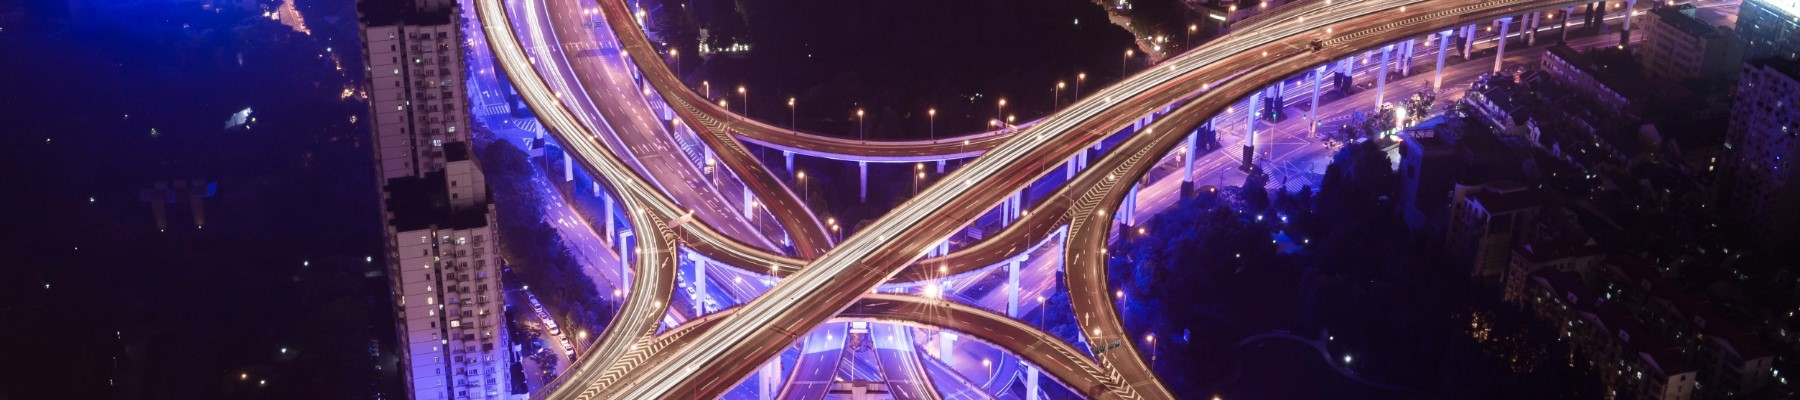
\includegraphics[width=\textwidth]{paperteaser3}
\end{teaserfigure}


% Disable automatic indentition after new paragraph
\setlength{\parindent}{0pt}

\maketitle

x\section{Einführung}

Das allgemeine Verkehrsaufkommen in Städten steigt seit Jahren konstant an. Die damit einhergehenden Herausforderungen, sowohl für die Verkehrslenkung selbst, als auch für das gesamtstädtische Leben, bringen konventionelle Betriebsmodelle an ihre Grenzen. Das Diginet-PS bietet eine Infrastruktur um bekannte Probleme durch neue, agententechnologische Ansätze zu lösen. Im Folgenden stellen wir Use-Cases vor um der Diginet-PS durch Agententechnologien einen Mehrwert zu bieten.

\section*{Use-Case 1: Dynamische Ampelschaltungen}

Ampeln sind ein unerlässliches Element um eine sichere Verkehrslenkung zu gewährleisten. Die Intervalle der Ampelschaltungen sind integraler Bestandteil der innerstädtischen Verkehrsflussplanung. Konventionelle Ampelanlagen sind in der Regel statisch geschaltet, d.h. die Intervalle der Ampelphasen sind fix und passen sich, wenn überhaupt, der gegebenen Tageszeit an. Zwar existieren insbesondere im urbanen Gebiet auch dynamisch geschaltet Anlagen (z.B. mittels funkgetriebener Vorrangschaltung für ÖPNV), eine dynamische Anpassung der Schaltintervalle an das aktuelle Verkehrsaufkommen findet jedoch nicht statt. \\

Durch agententechnologische Ansätze, lassen sich Ampeln in Echtzeit und adaptiv zum aktuellen Verkehrsfluss schalten. Das Diginet-PS wird dafür um einen Brokerservice erweitert, wobei die gesamte Fläche des Diginet in mehrere Areale aufgeteilt wird. Für jedes Areal ist ein Broker zuständig. Eine Ampelanlage fragt nach Ablauf einer kurzen, fest definierten Zeitspanne (z.B. fünf Sekunden) den für das jeweilige Areal zuständigen Broker an (\textit{Polling}). Der Broker sendet daraufhin eine Anfrage an alle Transportagenten im Areal. Diese melden zurück, ob gerade an der jeweiligen Ampel gewartet-, oder sich auf diese zubewegt wird. Auf diese Weise ermittelt der Broker, wie viele Verkehrsteilnehmer, in welche Richtung die Kreuzung überqueren möchten. Anhand des gemeldeten Verkehrsaufkommens kann die Ampelschaltung nun die optimalen Intervalle der Ampelphasen berechnen und einen maximalen Verkehrsfluss gewährleisten.\\

Insbesondere an Kreuzungen zwischen einer weniger genutzen und einer viel befahrenen Straße, wird sich der Verkehrsfluss deutlich verbessern. Die Schaltung einer \textit{grünen Welle}, geschieht durch unseren Ansatz im Idealfall von selbst, wodurch sich eine nennenswerte Energieersparnis bei allen Verkehrsteilnehmern erreichen lässt. Auf vielbefahrenen Kreuzungen mit einem gleichmäßigem Verkehrsaufkommen entsteht dagegen ein enorm hohes Datenaufkommen, ohne dass unser Ansatz einen großen Mehrwert gegenüber der statischen Schaltung bieten würde. Deshalb sollen die Ampeln bei anhaltender Gleichverteilung des Verkehrs das \textit{Polling-Intervall} erhöhen und sich bei der Berechnung des Schaltintervalls an vorherigen Messungen orientieren. 

\section*{Use-Case 2: Intelligente Straßenbeleuchtung}
Neben der Optimierung von Wartezeiten an Ampeln lässt sich durch neuartige Ansätze mit Agententechnologien auch großflächig Strom sparen. In Deutschland wird jährlich 0,8 \% des gesamten Strombedarfs durch Straßenlaternen aufgenommen. Gleichzeitig ist eine andauernde Ausleuchtung bei voller Helligkeit ineffizient, da die meisten Straßen nachts nur selten genutzt werden. Eine Umsetzung einer on-demand-Ausleuchtung eines Straßenabschnittes birgt daher enormes Einsparpotential. 
In diesem Szenario stellt ein Auto einen Agenten dar, eine Road-Side Unit mit einem dahinterstehenden Server den Broker und eine Laterne ist ein ausführender Agent.\\

Jedes Auto durch seine Navigationseinheit ein Wissen über die zukünftige Route. Mit diesen Informationen wird ein lokaler Broker mit einem fest definierten Zuständigkeitsbereich mit der Aufforderung angesprochen die nächsten n Laternen auf der Strecke als Empfehlung zu liefern. Der Broker wählt diese anhand der mitgeteilten Route aus und sendet diese als Antwort zurück an das Auto\textit{(Recommendation)}. Nun kann das Auto für den Zeitraum der vorbeifahrt die Ampeln auf volle Helligkeit schalten. Ansonsten befindet sich die Laterne in einem Energiesparmodus auf einem geringen Helligkeitsniveau. Auf diese Weise wird der Fahrtweg eines Autos immer ausreichend ausgeleuchtet.\\

Die Umsetzung mit Agententechnologien birgt hierbei den großen Vorteil, dass die Informationslast gleichmäßig über alle Teilnehmer verteilt ist. Ein zentrales System skaliert wesentlich schlechter, da hierbei ein zentraler Rechner Informationen über alle Laternen und Verkehrsteilnehmer vorhalten muss. Dies ist nicht nur ein hoher Verarbeitungsaufwand, sondern stellt auch einen \textit{single-point-of-failure} da. Weiterhin wird durch die direkte Kommunikation zwischen Auto und Laterne die Transmissionszeit von Nachrichten verkürzt und so ein höherer Grad an Reaktivität erreicht.\\

Die Effizienz dieses Ansatzes hängt stark von der Streckenauslastung ab. Falls das Verkehrsaufkommen so hoch ist, dass alle Lampen konstant verwendet werden, bringen die Kosten durch den Kommunikationsaufwand keinen Nutzen mehr. Gleichzeitig kann dies zu neuen stadtplanerischen Herausforderungen führen, da das ständige Flackern der Beleuchtung , ähnlich wie bei Windkraftanlagen, Anwohner schwerwiegend irritieren kann. Ein Fokus innerhalb der Projektlaufzeit wird daher auf die optimale Wahl von Regionen und Zeiten für den Einsatz dieser Technologie gelegt.

\section*{Use-Case 3: Optimale Parkplatzverteilung}
Der Verkehrsfluss ist nicht der einziger Bereich im städtischen Transport, wo der Einsatz von agentenorientierten Technologien eine Effizienzsteigerung erreichen kann. Zurzeit basiert die Vergabe von Parkplätzen in der Innenstadt grundsätzlich auf dem ``First Come, First Serve`` Prinzip. Bei mangelnder Information von Fahrern über die Parkmöglichkeiten verfolgt die Verteilung auf freie Parkplätze auf eine suboptimale Weise. Da große, intensiv benutzte Parkplätze zum Beispiel neben dem Mathe- oder Hauptgebäude der TU Berlin sowie entlang der Straße des 17 Juni und Querstraßen in der Umgebung  Teil der Diginet-PS Teststrecke sind, eignet sie sich besonders gut um die Umsetzung eines intelligenten Platzverteilungssystems für dieses Szenario unter realistischen Bedingungen zu untersuchen.\\

Das System basiert auf dem \textit{Contract Net Protocol}. Zu diesem Zweck wird das Diginet-PS um einen zentralen, autonomen Manager erweitert, der die Rolle des Initiators realisiert und für alle Parkplätze in Diginet Gelände zuständig ist. Seine Aufgabe ist es, die Stellen auf die Teilnehmer so zu verteilen, dass ihre persönliche Präferenzen bestmöglich erfüllt werden. Autos, bzw ihre Fahrer reichen Anfragen ein, wobei ihre Präferenzierung Kriterien wie das Vorhandensein von Lademöglichkeiten für Elektroautos oder eine behindertengerechte Platzierung widerspiegeln kann. Die Kosten, die ein Teilnehmer in einem Angebot einreicht, setzt sich aus dem Parkpreis und der Entfernung von der jetzigen und der geplanten Zielposition zusammen. Nachdem eine fest definierte Frist abgelaufen ist oder die Anzahl der Anfragen eine bestimmte Quote erreicht, werden sie vom Manager evaluiert und die Plätze werden möglichst optimal zugewiesen. Falls es mehr Anfragen als Parkplätze gibt, erhalten die Anfragen mit strengsten Kriterien eine Ablehnung. Dieses Verfahren kann auch in erweiterter Form mit mehreren Iterationen umgesetzt werden, damit die Anfragen erneut mit schwächeren Kriterien nachgereicht werden können.\\

Der Einsatz eines \textit{Contract Net Protocol} bringt viele Vorteile mit sich. Die Autofahrer können schon während der Reise mit mehreren Parkplatzmanagern handeln statt systematisch alle Parkplätze in der Umgebung durchsuchen. Körperlich behinderte Menschen sind besser informiert über die Verfügbarkeit der ihnen angepassten Parkstellen. Außerdem können die Fahrer, die nach billigsten beziehungsweise nächsten Plätzen suchen, besser ein möglichst geeignetes Angebot finden. Letztendlich sind die Parkplätze effizienter und gleichmäßiger ausgelastet.\\

Ein sehr wahrscheinliches Szenario bei der Parkplatzverteilung ist, wenn die Anzahl der Autos viel größer als Anzahl der verfügbaren Plätze ist und immer neue Anfragen zukommen. In diesem Fall ist die kurze Antwortzeit für die Fahrer besonders wichtig, weil die Wahrscheinlichkeit der Ablehnung höher ist und dadurch müssen sie durchschnittlich mehr Anfragen schicken um eine Parkstelle zu reservieren. Das Verfahren kann aber, besonders in iterativer Variante, lang dauern und die Fahrer die besonders nah zum Parkplatz sind und somit sehr große Chancen haben, warten genauso lang wie alle andere auf die Antwort, was für sie relativ großen Zeitverlust darstellt. Dann ist für sie das System im Nachteil im Vergleich zu traditioneller Suche nach einer Parkstelle. Diese Evaluation wird ein integraler Bestandteil der Projektarbeit werden und aufbauend darauf wird das effektivste System für die Strecke implementiert.







\end{document}
